\documentclass[11pt,a4paper]{article}
\usepackage{fontspec}
\setmainfont{TeX Gyre Pagella}
\newfontfamily\headfont{Inter}[UprightFont=*-ExtraBold,BoldFont=*-ExtraBold,Extension=.otf,Path=/usr/share/fonts/opentype/inter/]
\usepackage[a4paper,margin=2.3cm]{geometry}
\usepackage{graphicx,booktabs,float,caption,array,xcolor,longtable}
\usepackage{xurl}
\usepackage[hidelinks]{hyperref}
\usepackage{titlesec}
\usepackage[round]{natbib}
\usepackage{setspace}
\setstretch{1.05}
\renewcommand{\topfraction}{0.9}
\renewcommand{\bottomfraction}{0.8}
\renewcommand{\textfraction}{0.1}
\renewcommand{\floatpagefraction}{0.75}
\setlength{\parindent}{0pt}
\setlength{\parskip}{0.55em}
\titleformat{\section}{\headfont\Large}{\thesection}{0.8em}{}
\titleformat{\subsection}{\headfont\large}{\thesubsection}{0.8em}{}
\captionsetup{font=small,labelfont=bf}
\urlstyle{same}
\hypersetup{pdftitle={Which Way Do Cricket Pitches Face?},pdfauthor={Tristan Hotham}}

\begin{document}
\begin{center}
{\Large\bfseries Which Way Do Cricket Pitches Face?\par}
\vspace{0.4em}
{\large The orientation of 1,394 cricket strips and 61,215 other sports pitches\\in OpenStreetMap, the low sun and the street grid\par}
\vspace{1.2em}
{\large Tristan Hotham\par}
\vspace{0.3em}
{\small Independent researcher\\
ORCID: 0000-0003-4931-9349\\
DOI: https://doi.org/10.5281/zenodo.24075295\par}
\vspace{0.8em}
2026
\end{center}

\begin{quote}
\small
\begin{center}\textbf{Abstract}\end{center}
Design guidance advises that cricket pitches and tennis courts should run roughly north to south, so that the low sun does not shine along the line of play. I test whether real pitches follow the advice, using the outline of every cricket pitch mapped in OpenStreetMap worldwide (15,168 polygons) and every sports pitch in the United Kingdom (84,853). The long axis of each outline is the long side of its minimum-area enclosing rectangle in a local true-north frame. Cricket polygons are sorted by size and shape into single pitches (strips), blocks of strips (squares), whole grounds and practice nets, after checking samples by eye. Of 1,394 strips, 54.7\% lie within 20° of the north to south line, against 22.2\% expected by chance: 68.6\% in Australia, 46.9\% in the United Kingdom and 34.3\% in New Zealand. Among UK pitches, tennis courts follow the rule (40.5\%), while football (26.1\%), rugby (25.3\%) and Gaelic games (24.1\%) are close to chance, and football and rugby pitches are about as often east to west as north to south. A simple model of low sun along the line of play shows a wide glare-free arc around north to south (at 52°N, from -33° to 61° from north), which holds 82.5\% of strips. In built-up places where the street grid turns away from the compass, most pitches follow the streets, but cricket strips do so least often (66.3\%, against 84.9\% of football pitches).

\textbf{Keywords:} sports pitches; cricket; orientation; sun glare; OpenStreetMap; street networks; sports facility design
\end{quote}

\section{Introduction}
Design guidance says that a cricket pitch should be laid roughly north to south. The sports dimensions guide of the Government of Western Australia, for example, states that cricket pitches must run approximately north to south to minimise the risk of batters or bowlers facing a low sun, and that tennis courts must be oriented with play along an approximately north to south axis \citep{wa}. Cricket is played through long summer afternoons and evenings, and when the sun is low in the west a pitch running east to west puts it in the eyes of the batter at one end and the bowler at the other. For football, FIFA's stadium guidelines note that the most common orientation of a pitch or stadium is predominantly north to south \citep{fifa}, but those guidelines are written for stadiums; whether ordinary club and park pitches follow any such rule is an open question.

Whether pitches actually follow the advice has, as far as I know, not been measured at scale. OpenStreetMap \citep{osm} now holds the outlines of tens of thousands of sports pitches, which makes it possible to ask, for every mapped pitch at once: how far does it turn from north to south, does cricket differ from other sports, does the share change with country and latitude, and is the local street grid a better guide? The method follows a study of church orientation from the same data \citep{churches}. The study accompanies an interactive map of every measured pitch (\url{https://maps.tristanhotham.com/pitch-orientation/}).

\section{Data}
\textbf{Pitches.} Two extracts were made with the QLever SPARQL engine \citep{qlever} over the osm2rdf conversion of OpenStreetMap \citep{osm2rdf}: every way or relation in the United Kingdom tagged \texttt{leisure=pitch} with a \texttt{sport} tag (84,853 polygons; Table~\ref{tab:sports} gives the counts by sport), and every way in the world tagged \texttt{leisure=pitch} and \texttt{sport=cricket} (15,168 polygons in 105 countries, 4,150 of them in the United Kingdom). Points were dropped. The country of each cricket pitch comes from the Natural Earth 1:10m boundaries \citep{ne}.

\textbf{Streets.} Road centrelines around a sample of pitches were read from the OpenFreeMap vector tiles \citep{ofm} at zoom 14 (OpenMapTiles schema, OpenStreetMap data).

\section{Methods}
\subsection{The axis}
Each outline (the largest polygon of a multipolygon) is projected to a local equirectangular frame about its own centroid, which keeps true north up. The minimum-area enclosing rectangle \citep{freeman} gives the axis: the bearing of its long side, folded into 0° to 180°. The turn from north to south is the smaller angle between that axis and the meridian (0° to 90°). A random axis lies within 20° of north to south with probability $40/180 = 22.2\%$ and within 30° with probability 33.3\%; shares are tested against these with an exact binomial test. The axial mean doubles the angles, averages the unit vectors and halves the result; its length $R$ measures agreement.

\subsection{What a cricket pitch is}
The \texttt{leisure=pitch} tag is used for three different things in cricket, and they have to be separated (Figure~\ref{fig:shapes}).
A \emph{strip} is a single pitch: the 22 yards (20.12 m) between the wickets with its creases. Strips are rectangles 17 to 45 m long, 1.5 to 6 m wide and at least 3.5 times as long as wide; the median strip measures 25.9 m by 2.9 m. Its long axis is the line of play.
A \emph{square} is the block of turf in the middle of a club ground holding a dozen or so strips side by side: here, any outline of 180 to 3,500 m² and at most 60 m long that fills at least 85\% of its rectangle. Its strips may run along either side, so for squares only the turn from the compass (folded modulo 90°) is used.
A \emph{ground} is the whole field, 6,000 m² or more, usually round or oval. Grounds have no axis; only grounds at least 1.2 times as long as wide are given one, as a weak proxy. Of the 85 strips mapped inside a ground, those in such elongated grounds lie within 20° of the ground's long axis in 81.8\% of cases (n = 33, median difference 2.8°), against 32.7\% for rounder grounds.
\emph{Nets}, for practice, are kept apart: outlines named as nets or practice areas (227), rectangles of strip length but 6 to 12 m wide (310), and strips lying just outside a mapped ground, within 40 m of its edge (25). The last two rules came from checking contact sheets, which drew every strip of a random sample of 120 with the roads and buildings around it from the OpenFreeMap tiles: about 10 were banks of nets beside a ground rather than the pitch in its middle. The rules moved 19.4\% of the first list of 1,729 strips to nets. A second sample of 60 strips, drawn after the rules, held 1 doubtful case. Two polygons of the same class overlapping by 80\% or more were treated as one (2 cricket duplicates).

\subsection{Other sports}
For other sports, an outline is measured only when its rectangle has the size and shape of one playing area: football 30 to 130 m long and 1.25 to 2.2 times as long as wide; rugby 60 to 160 m and 1.3 to 2.3; hockey 40 to 110 m; Gaelic games 80 to 170 m; tennis 22 to 42 m long, 10 to 21 m wide and 1.6 to 2.6 times as long as wide; netball 24 to 40 m; basketball 20 to 40 m. This drops blocks of several courts side by side, whose long side runs across the courts, and odd shapes. Bowling greens are square and have no axis. Athletics features mapped as pitches are mostly jump runways and throwing circles and are left out.

\subsection{The glare model}
For a pitch at latitude $\varphi$ with its line at bearing $b$, the model counts the minutes in a cricket season when the sun's apparent altitude is above 0° and at most 15°, and its azimuth is within 15° of $b$ or $b+180°$, between 10:00 local apparent solar time and sunset. The solar declination follows \citet{spencer}, the position follows from the hour angle minute by minute, and refraction from \citet{bennett}. The season is mid April to mid September north of the tropics, mid October to mid March in the southern hemisphere and the northern tropics. The glare-free arc is the set of bearings with no such minutes. The model ignores trees, stands, cloud and real fixtures, and is meant only to show which directions the low sun can reach.

\subsection{The street grid}
For every strip and square, and random samples of UK football pitches (2,500), tennis courts (2,500), rugby pitches (800) and netball and basketball courts, the road centrelines from motorways to service roads (paths and tracks excluded) within 200 m of the centroid were collected. The local grid direction is the length-weighted dominant direction of the segments folded modulo 90°, a simple form of the street orientation measures of \citet{boeing}. A pitch counts as built-up when there are at least 1,500 m of road within the circle. Where the grid turns at least 15° from the compass, so that the two can be told apart, the angles of the pitch to the grid and to the compass (both folded to 0° to 45°) are compared. A pitch at a random direction would be closer to the grid than to the compass half the time, so 50\% is the baseline for this comparison. Road segments are counted whole when any part of them lies within the circle.

\section{Results}
\subsection{Cricket strips}
Of the 1,394 strips, 54.7\% lie within 20° of north to south and 66.4\% within 30°, while 9.9\% lie within 20° of east to west (Figure~\ref{fig:map}). The axial mean is 3.3° with $R = 0.49$. The result does not depend on grounds with many strips: grouping strips within 120 m into 1,197 grounds and giving each one vote, 53.6\% lie within 20°. In the United Kingdom, where strips are seldom mapped, squares add evidence: 31.8\% of 578 UK squares have their long side within 20° of east to west and 16.6\% within 20° of north to south. A square is usually wider across its strips than along them (though not always: a narrow square of a few strips can be longer along them), so this fits strips running north to south, but it is weaker evidence than the strips themselves.

\begin{figure}[tbp]\centering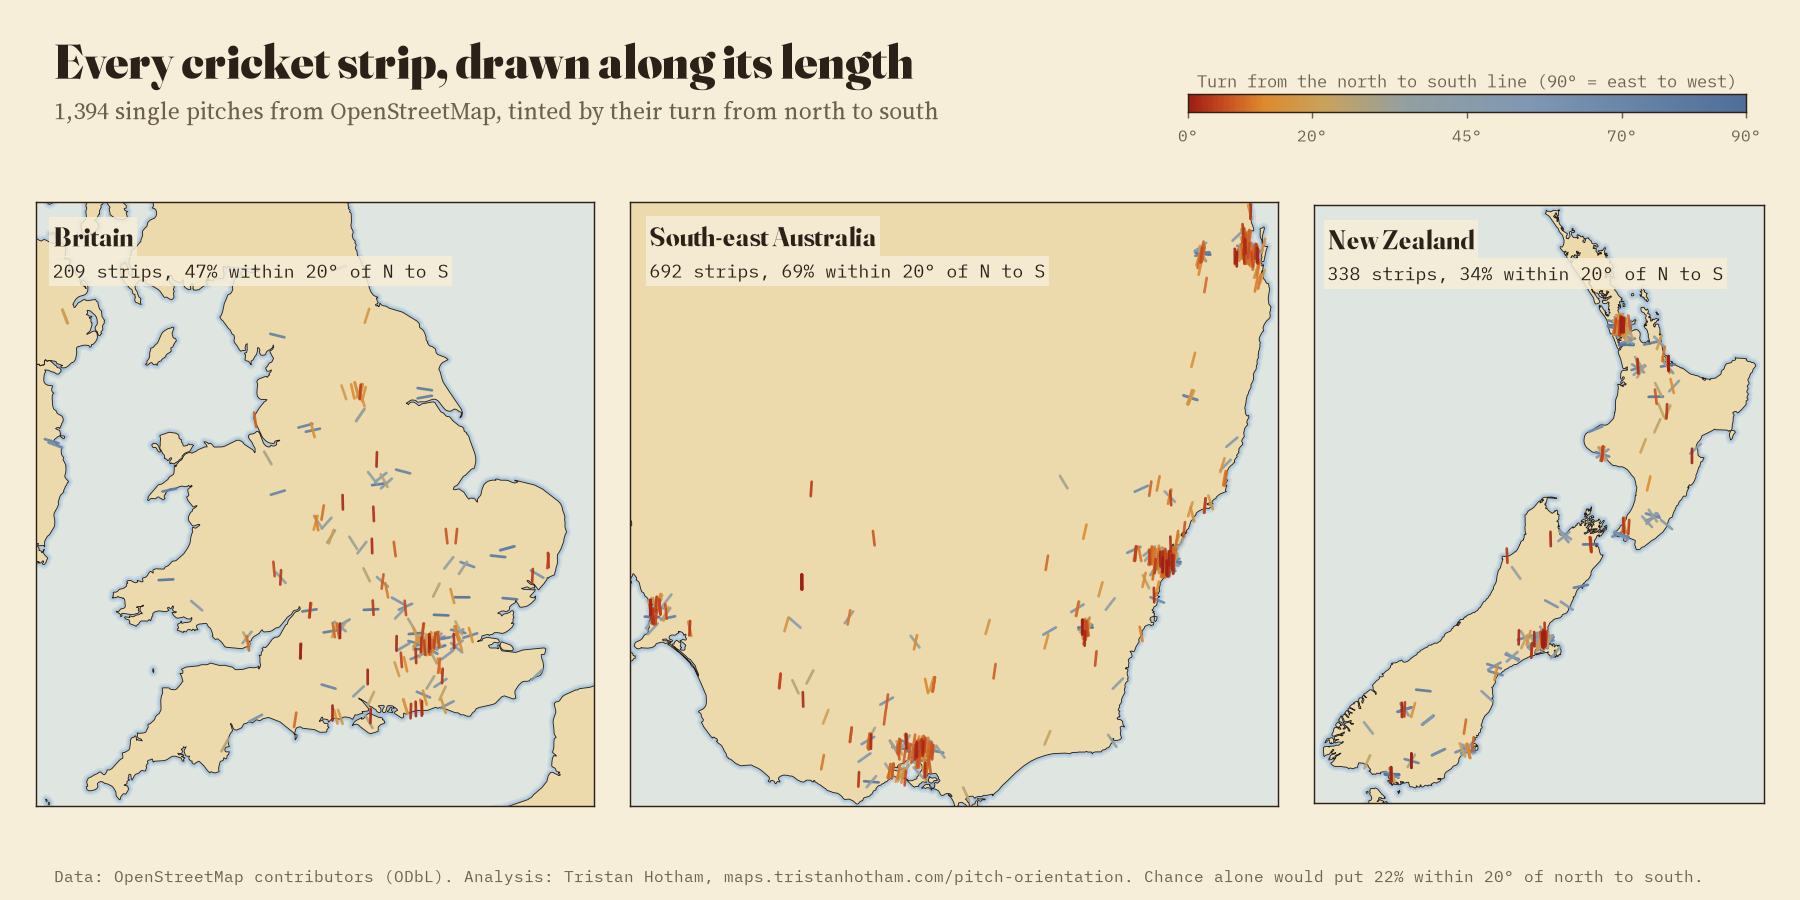
\includegraphics[width=\textwidth]{f_map.png}
\caption{Every mapped strip in Britain, south-east Australia and New Zealand, coloured by its turn from north to south.}\label{fig:map}\end{figure}
\begin{figure}[tbp]\centering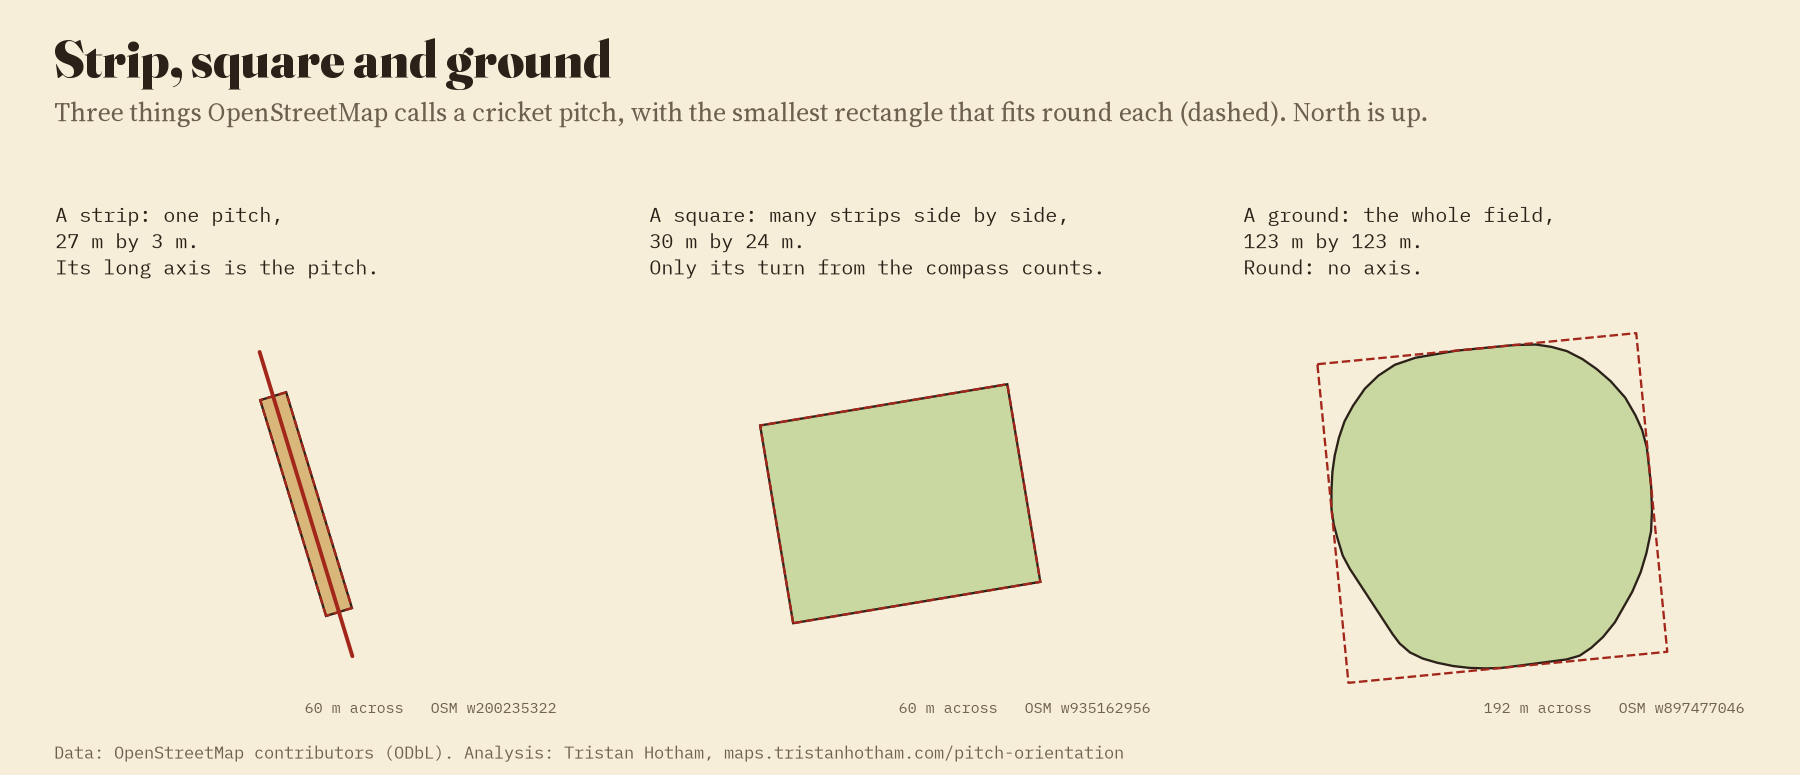
\includegraphics[width=\textwidth]{f_shapes.png}
\caption{A strip, a square and a ground, with their minimum-area rectangles.}\label{fig:shapes}\end{figure}

\subsection{Other sports}
Table~\ref{tab:sports} and Figures~\ref{fig:sports} and~\ref{fig:roses} compare sports in the United Kingdom. Tennis courts are the only other sport close to cricket: 40.5\% within 20° of north to south and 12.1\% within 20° of east to west. Netball reaches 30.0\%. Football (26.1\% north to south, 25.3\% east to west) and rugby (25.3\%, 24.3\%) show a slight excess over chance in both directions at once, as pitches laid square to rectangular fields would, but no clear preference for north to south; Gaelic games (24.1\% and 19.8\%, n = 349) do not differ clearly from chance.

\begin{table}[tbp]\centering\small\caption{United Kingdom, pitches with an axis by sport: number measured; share (\%) within 20° and 30° of north to south and within 20° of east to west; axial mean bearing (degrees from north, negative west of north) and its length $R$; binomial p-value for the 20° share against 22.2\%. Polygons tagged in the UK file: football 25,319, tennis 35,208, cricket 4,152, rugby 3,667.}\label{tab:sports}\begin{tabular}{lrrrrrrr}\toprule Sport & n & $\le$20° & $\le$30° & E to W $\le$20° & Mean & $R$ & p\\\midrule
Cricket strips & 209 & 46.9 & 60.8 & 15.3 & -1.8 & 0.36 & $<$0.001\\
Tennis & 29,426 & 40.5 & 55.9 & 12.1 & -3.6 & 0.35 & $<$0.001\\
Netball & 1,258 & 30.0 & 40.5 & 21.0 & 11.2 & 0.10 & $<$0.001\\
Hockey & 646 & 28.2 & 39.0 & 22.1 & -5.2 & 0.07 & $<$0.001\\
Basketball & 2,932 & 26.6 & 38.2 & 23.3 & -11.8 & 0.05 & $<$0.001\\
Football & 23,114 & 26.1 & 37.3 & 25.3 & -14.2 & 0.02 & $<$0.001\\
Rugby (union, league) & 3,490 & 25.3 & 37.0 & 24.3 & -20.4 & 0.01 & $<$0.001\\
Gaelic games & 349 & 24.1 & 37.2 & 19.8 & 9.3 & 0.04 & 0.221\\
Cricket squares (long side) & 578 & 16.6 & 27.3 & 31.8 & -86.4 & 0.20 & 1.000\\
Cricket nets & 119 & 36.1 & 47.9 & 16.0 & 3.2 & 0.20 & $<$0.001\\
\bottomrule\end{tabular}\end{table}

\begin{figure}[tbp]\centering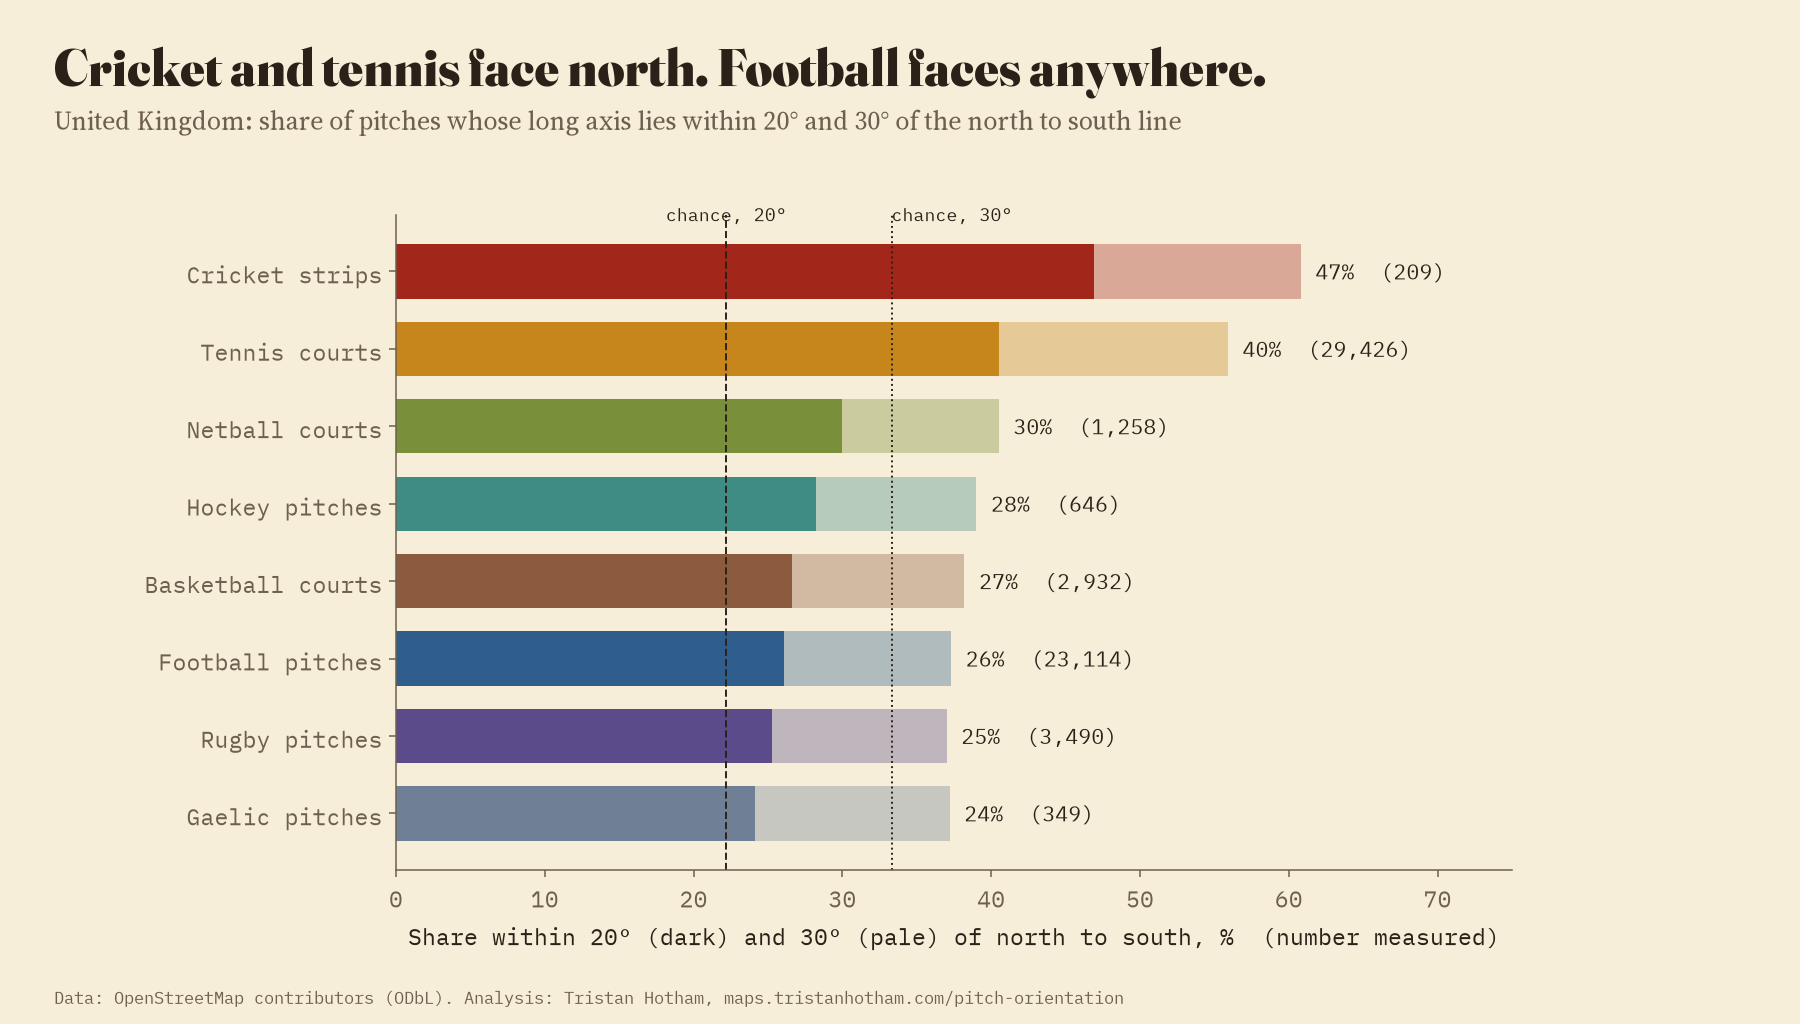
\includegraphics[width=0.92\textwidth]{f_sports.png}
\caption{United Kingdom: share of pitches within 20° (dark) and 30° (pale) of north to south, by sport.}\label{fig:sports}\end{figure}
\begin{figure}[tbp]\centering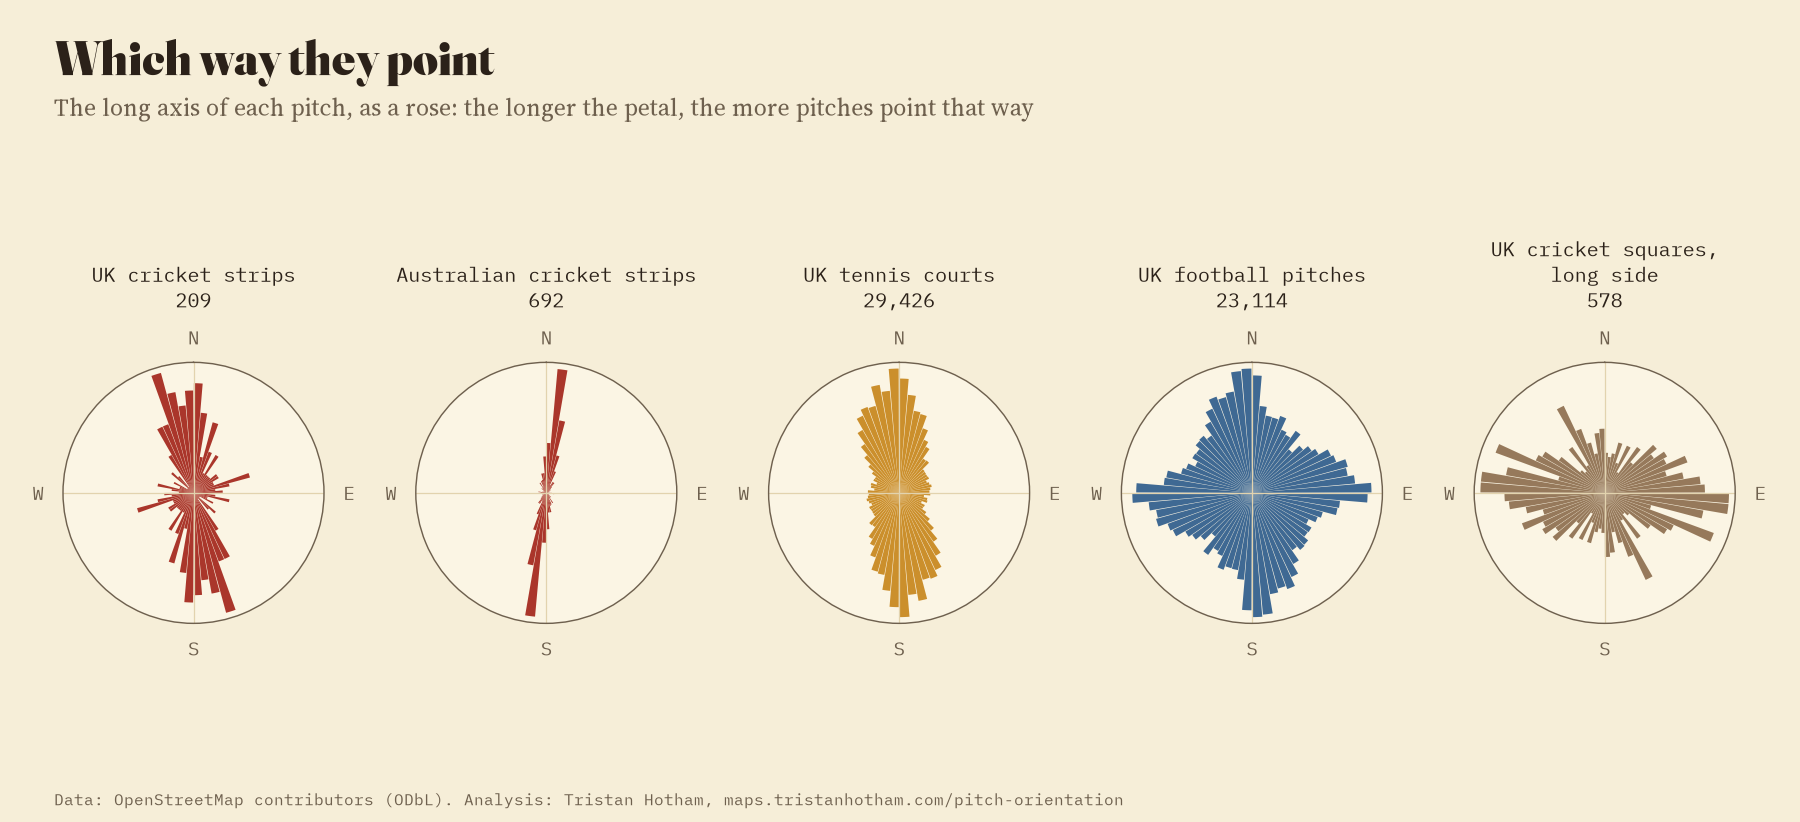
\includegraphics[width=\textwidth]{f_roses.png}
\caption{Rose diagrams of pitch axes.}\label{fig:roses}\end{figure}

\subsection{Countries and latitude}
Table~\ref{tab:countries} and Figure~\ref{fig:countries} compare countries. Among the six with at least 20 strips, Australia has the highest share (68.6\% of 692, $R = 0.68$) and New Zealand among the lowest (34.3\% of 338). Strips in the southern hemisphere reach 56.6\% and in the northern 48.2\%. In India, Pakistan, Sri Lanka, Bangladesh and the Caribbean strips are rarely mapped, so the comparison the question invites (higher sun, shorter twilight) cannot be made fairly; elongated grounds in India lie within 20° of north to south in 43.1\% of 341 cases, and Indian squares are set within 10° of the compass in 46.8\% of 111.

\begin{table}[tbp]\centering\small\caption{Cricket by country: median latitude, all cricket polygons, strips and their share (\%) within 20° of north to south, squares and their share within 10° of the compass, elongated grounds and their share within 20° of north to south (shares shown for 10 or more). Caribbean: the West Indies cricket territories together.}\label{tab:countries}\begin{tabular}{lrrrrrrrr}\toprule Country & Lat. & All & Strips & $\le$20° & Squares & $\le$10° & Grounds & $\le$20°\\\midrule
United Kingdom & 52 & 4,150 & 209 & 46.9 & 578 & 27.9 & 763 & 27.7\\
Australia & -34 & 6,247 & 692 & 68.6 & 217 & 50.2 & 1515 & 57.5\\
New Zealand & -38 & 994 & 338 & 34.3 & 79 & 31.6 & 83 & 33.7\\
United States & 40 & 259 & 41 & 48.8 & 15 & 46.7 & 52 & 42.3\\
Canada & 44 & 139 & 22 & 45.5 & 3 & . & 15 & 53.3\\
Samoa & -14 & 53 & 24 & 29.2 & 3 & . & 6 & .\\
India & 20 & 1,397 & 17 & 52.9 & 111 & 46.8 & 341 & 43.1\\
South Africa & -30 & 526 & 13 & 46.2 & 35 & 28.6 & 129 & 34.9\\
Pakistan & 29 & 285 & 3 & . & 12 & 16.7 & 69 & 29.0\\
Sri Lanka & 7 & 166 & 1 & . & 2 & . & 65 & 26.2\\
Bangladesh & 24 & 102 & 2 & . & 4 & . & 32 & 56.2\\
Caribbean & 13 & 234 & 1 & . & 7 & . & 76 & 35.5\\
\bottomrule\end{tabular}\end{table}

\begin{figure}[tbp]\centering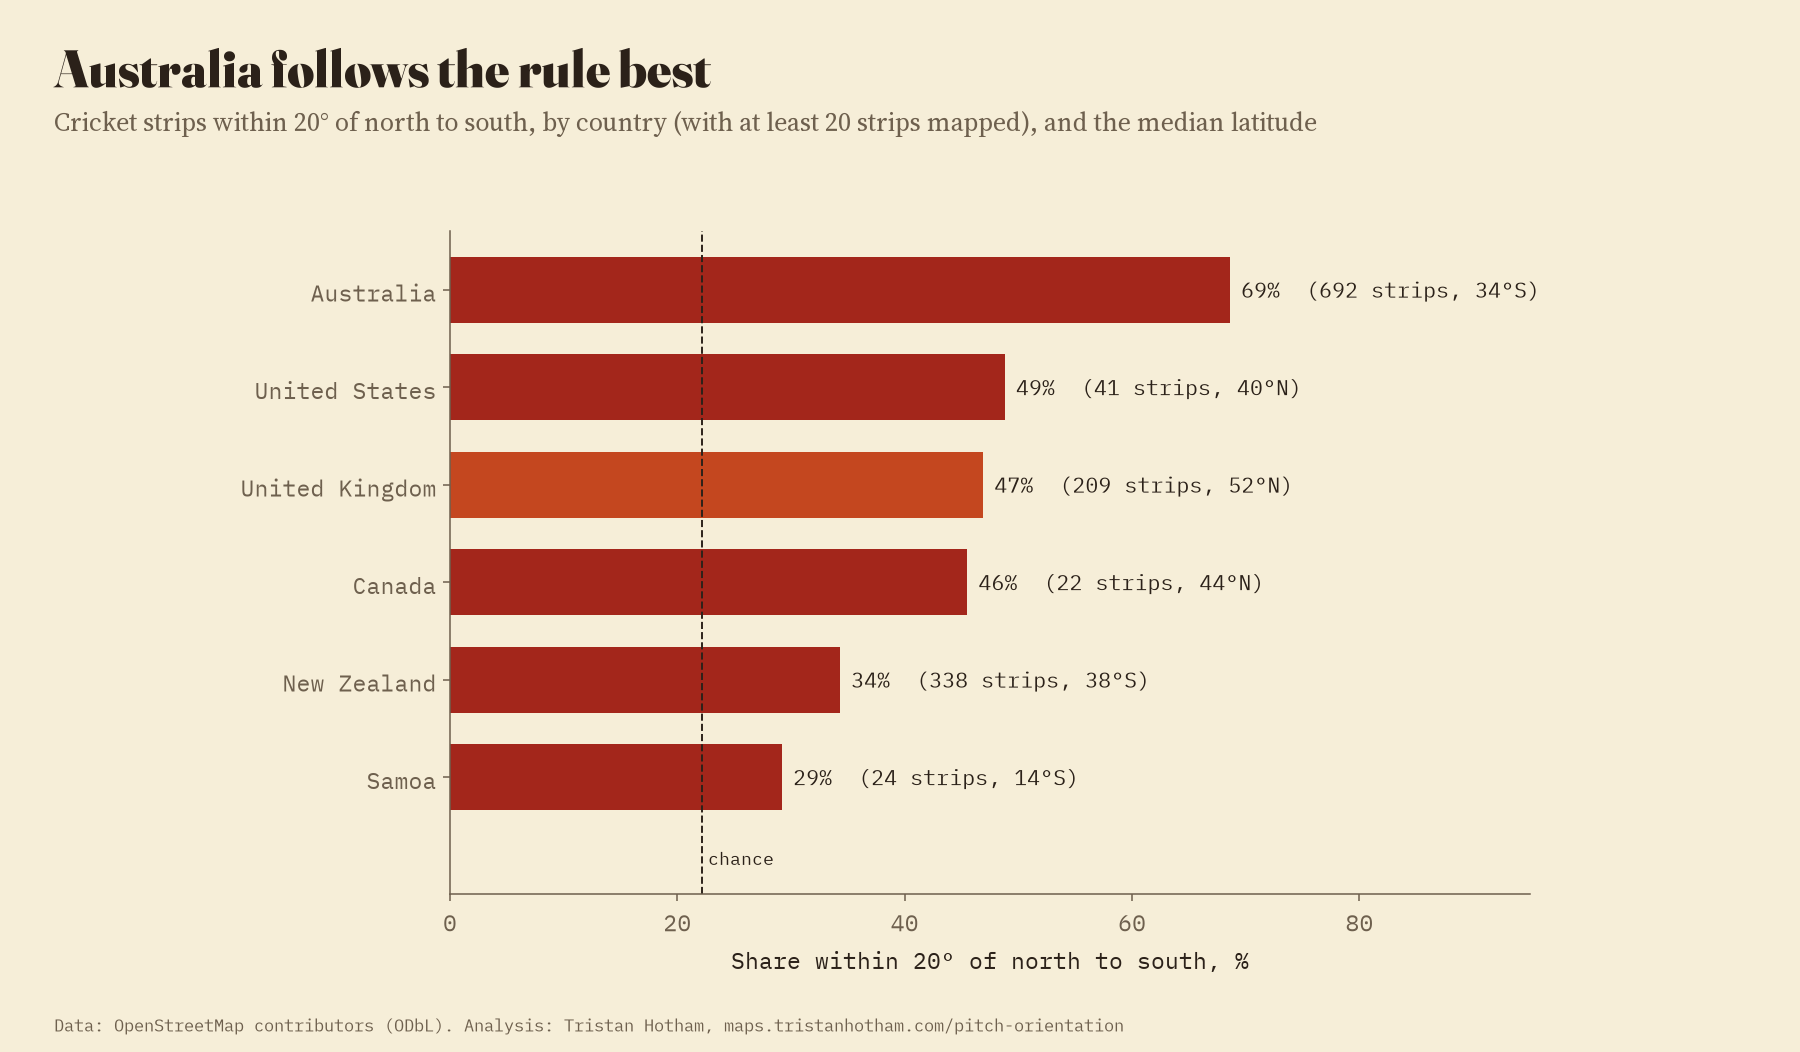
\includegraphics[width=0.92\textwidth]{f_countries.png}
\caption{Share of strips within 20° of north to south, countries with at least 20 strips.}\label{fig:countries}\end{figure}

\subsection{The sun}
The glare model (Figure~\ref{fig:glare}) shows why north to south is safe and how much room there is. At 52°N in an English season, a pitch running east to west has about 88 hours a season of low sun along its line, and the worst direction is 111° (east-south-east to west-north-west), towards the summer evening sun; every bearing from -33° to 61° from north has none. At 34°S the arc runs from -67° to 45°. The arc is wide, so the rule as practised is stricter than the sun requires: 73.7\% of UK strips lie in the glare-free arc for their latitude, against 52.8\% for a random direction, and 82.5\% of all strips do. The model's arcs lean east of north in the northern hemisphere and west of north in the southern; the axial means of strips do not clearly follow (United Kingdom -1.8°, Australia 6.6°, New Zealand -4.7°): pitches follow the rule, not the model.

\begin{figure}[tbp]\centering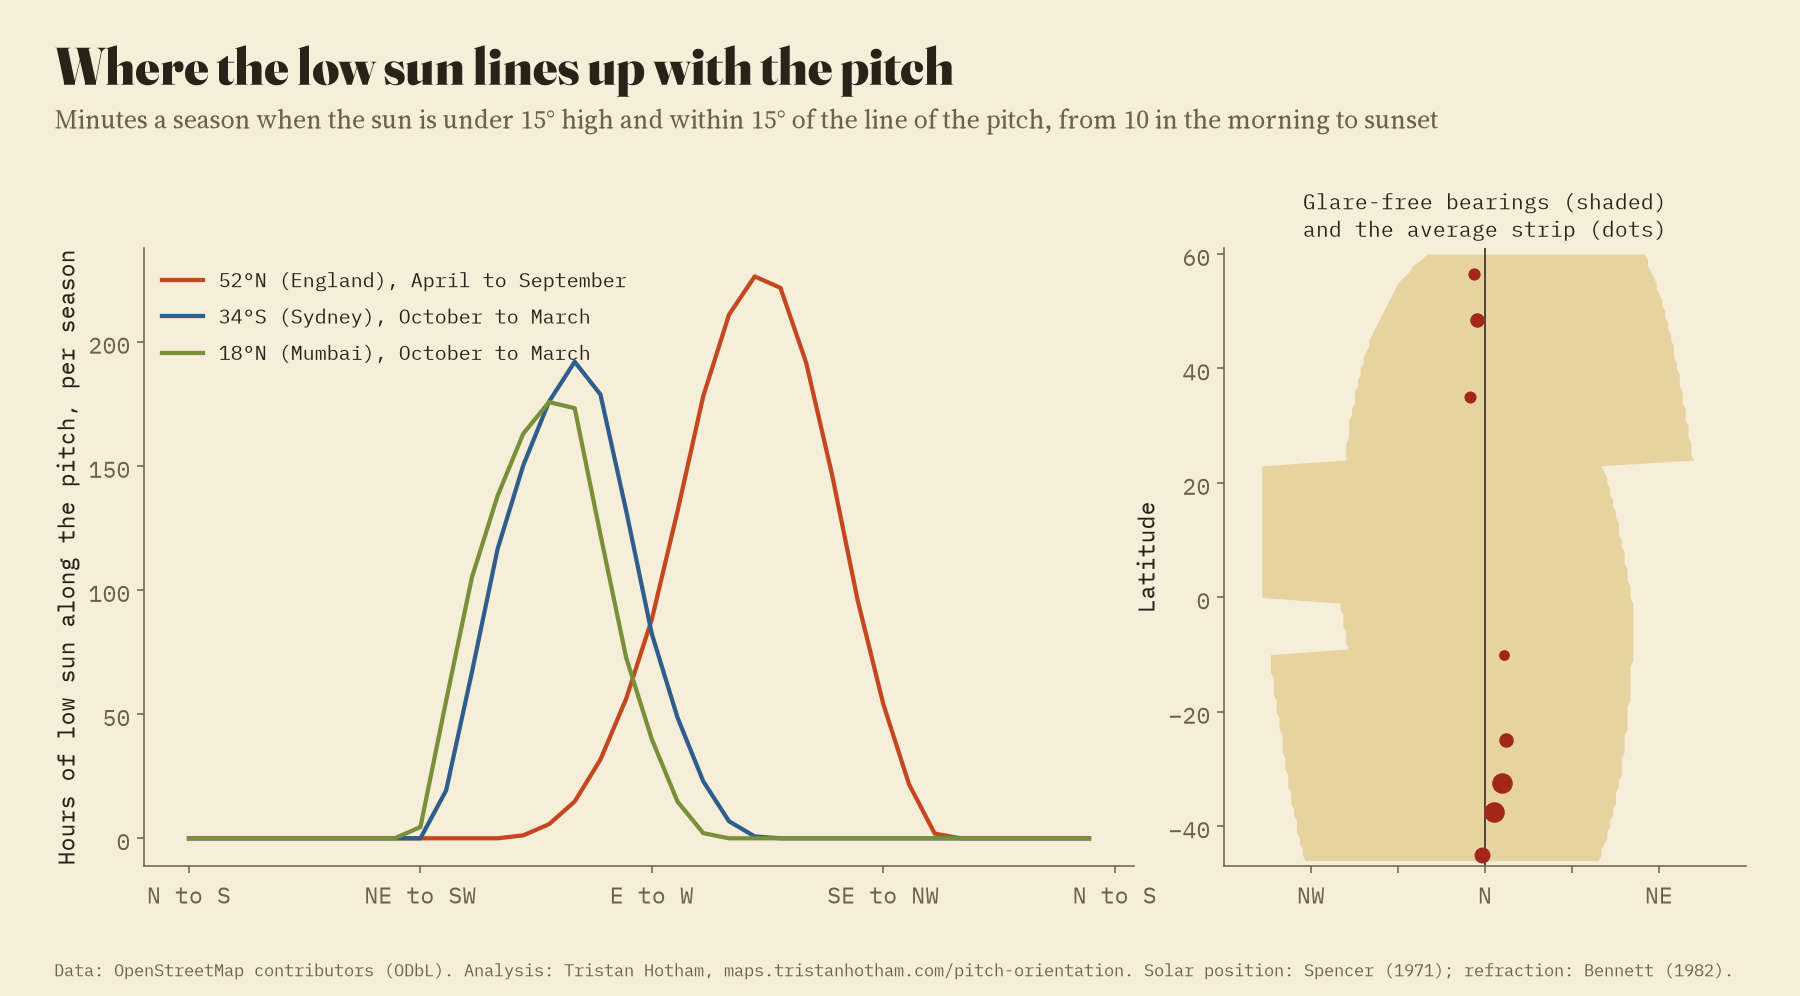
\includegraphics[width=\textwidth]{f_glare.png}
\caption{The glare model: hours of low sun along the pitch per season by pitch direction at three latitudes (left), and the glare-free arc by latitude with the axial mean of strips in latitude bands (right).}\label{fig:glare}\end{figure}

\subsection{The street grid}
In built-up places where the street grid turns at least 15° from the compass (Figure~\ref{fig:streets}), pitches are closer to the grid than to the compass in most cases: football 84.9\% (n = 823), rugby 90.2\% (n = 225), netball 85.1\%, basketball 81.7\%, tennis 80.0\% (n = 616), cricket squares 76.3\% (n = 346) and cricket strips 66.3\% (n = 398; Australia 53.2\%, n = 171; United Kingdom 82.5\%, n = 57). Within 5° of the grid lie 47.0\% of football pitches and 36.4\% of strips. The grid is a strong guide for every sport, but cricket strips resist it most, which is what the sun advice would predict.

\begin{figure}[tbp]\centering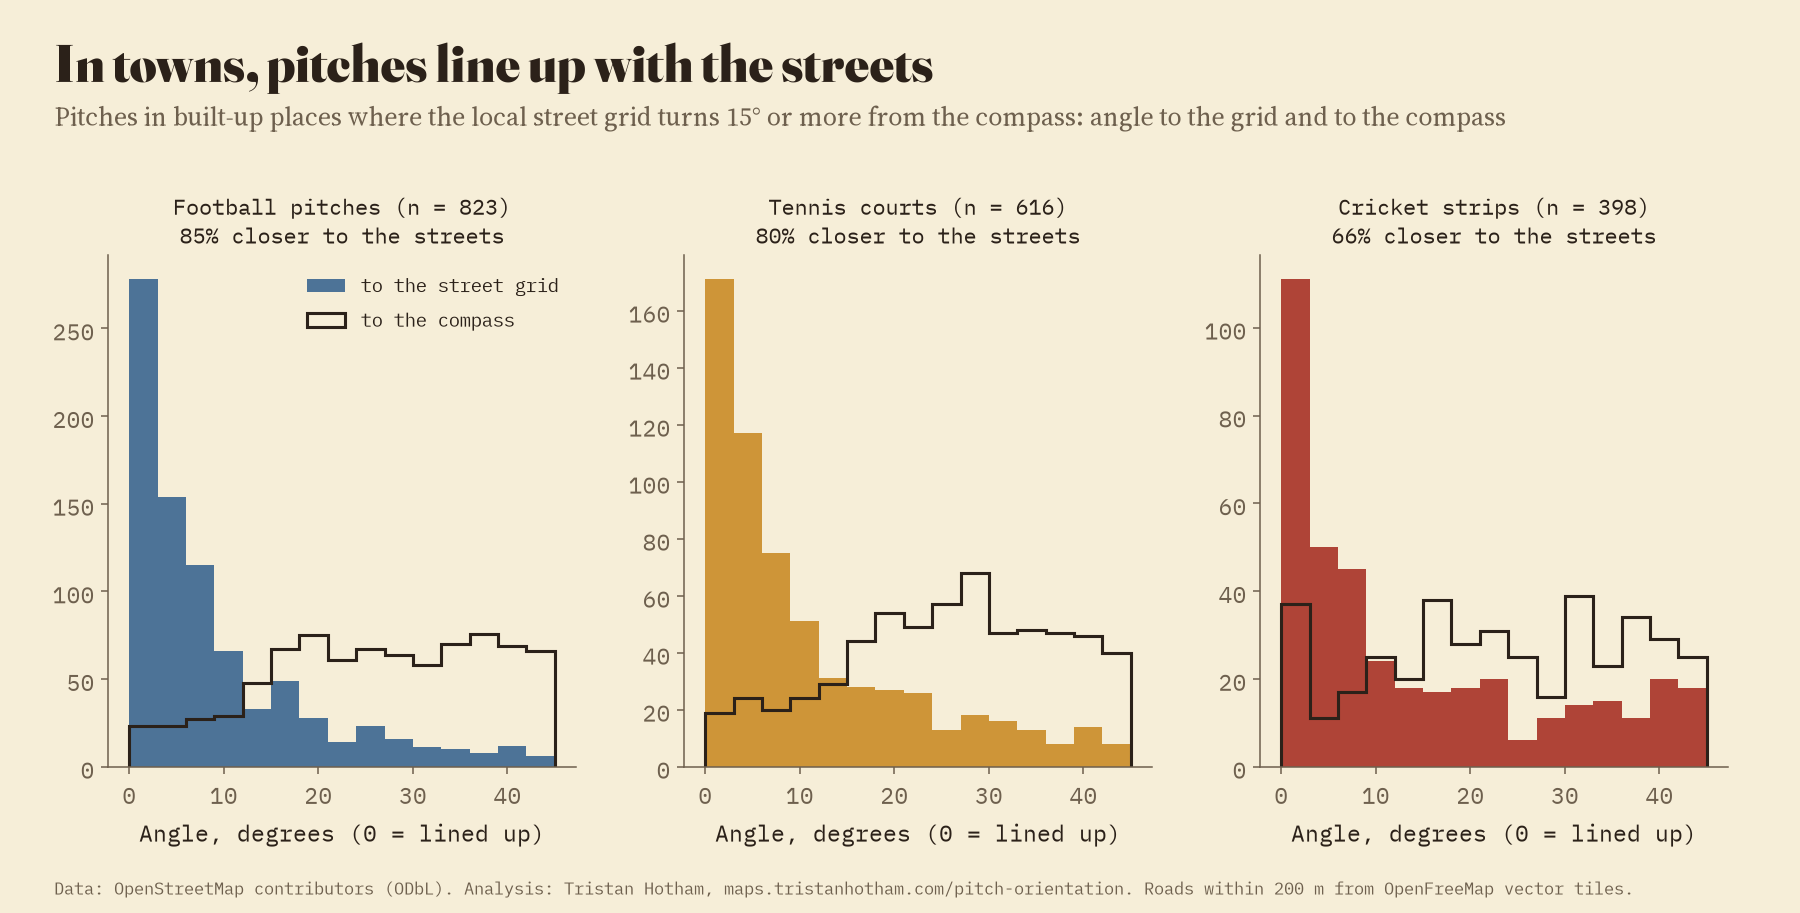
\includegraphics[width=\textwidth]{f_streets.png}
\caption{Pitches in built-up places with an off-compass grid: angle to the street grid (bars) and to the compass (line), folded to 0° to 45°.}\label{fig:streets}\end{figure}

\section{Limitations}
OpenStreetMap is uneven. Cricket strips are mapped mostly in Australia, New Zealand and Britain, and hardly at all in South Asia and the Caribbean, where most cricket is played; famous Test grounds are usually mapped as stadiums and are not in the data. The size rules are a compromise: a few single-lane nets will pass as strips, a few wide strips will have been called nets, and a mapper's rectangle may include the run-ups. The square's axis is ambiguous by nature. The street test uses today's roads and a fixed radius, and the association can run both ways: a new estate may be laid out around an older ground. The glare model is deliberately simple. Nothing here says who laid out a pitch or when.

\section{Conclusion}
Cricket strips do run north to south, more often in Australia than in Britain and New Zealand, and much more often than football or rugby pitches, which follow the fields they were fitted into. Tennis courts follow the same rule as cricket. The low sun leaves a wider arc of safe directions than the rule uses, so the rule is kept as a rule. In towns most pitches line up with the streets, cricket least of all.

\section*{Data and code availability}
The interactive map is at \url{https://maps.tristanhotham.com/pitch-orientation/}. Data and code are at \url{https://github.com/Tristan-Hotham/pitch-orientation} and archived with this paper at https://doi.org/10.5281/zenodo.24075295. The pitch table is derived from OpenStreetMap and released under the Open Database Licence; code is MIT licensed; text and figures CC BY 4.0.

\section*{AI statement}
I wrote the text, with drafting and editing assistance from Claude (Anthropic), which also helped prepare the analysis code. I reviewed and checked all text and results.

\begin{thebibliography}{99}
\bibitem[Bast and Buchhold(2017)]{qlever} Bast, H. and Buchhold, B. (2017) QLever: a query engine for efficient SPARQL+text search. In \textit{Proceedings of the 26th ACM International Conference on Information and Knowledge Management (CIKM 2017)}, 647 to 656. \url{https://doi.org/10.1145/3132847.3132921}
\bibitem[Bast et al.(2021)]{osm2rdf} Bast, H., Brosi, P., Kalmbach, J. and Lehmann, A. (2021) An efficient RDF converter and SPARQL endpoint for the complete OpenStreetMap data. In \textit{Proceedings of the 29th International Conference on Advances in Geographic Information Systems (SIGSPATIAL 2021)}. \url{https://doi.org/10.1145/3474717.3484256}
\bibitem[Bennett(1982)]{bennett} Bennett, G. G. (1982) The calculation of astronomical refraction in marine navigation. \textit{Journal of Navigation} 35(2), 255 to 259.
\bibitem[Boeing(2019)]{boeing} Boeing, G. (2019) Urban spatial order: street network orientation, configuration, and entropy. \textit{Applied Network Science} 4, 67. \url{https://doi.org/10.1007/s41109-019-0189-1}
\bibitem[FIFA(2022)]{fifa} FIFA (2022) \textit{FIFA Stadium Guidelines}, section 2.2, Orientation. Zurich: FIFA. \url{https://publications.fifa.com/en/football-stadiums-guidelines/}
\bibitem[Freeman and Shapira(1975)]{freeman} Freeman, H. and Shapira, R. (1975) Determining the minimum-area encasing rectangle for an arbitrary closed curve. \textit{Communications of the ACM} 18(7), 409 to 413.
\bibitem[Government of Western Australia(2025)]{wa} Government of Western Australia, Department of Creative Industries, Tourism and Sport (2025) \textit{Sports dimensions guide}. \url{https://www.cits.wa.gov.au/sport-and-recreation/sports-dimensions-guide}
\bibitem[Hotham(2026)]{churches} Hotham, T. (2026) Which way do the UK's churches face? The axes of church footprints from OpenStreetMap and a test of the patron saint's sunrise. Zenodo. \url{https://doi.org/10.5281/zenodo.24052501}
\bibitem[Natural Earth(2026)]{ne} Natural Earth (2026) Admin 0 countries, 1:10m. Public domain. \url{https://www.naturalearthdata.com/}
\bibitem[OpenFreeMap(2026)]{ofm} OpenFreeMap (2026) Free vector tiles (OpenMapTiles schema) from OpenStreetMap data. \url{https://openfreemap.org/}
\bibitem[OpenStreetMap contributors(2026)]{osm} OpenStreetMap contributors (2026) OpenStreetMap. Open Database Licence. \url{https://www.openstreetmap.org/}
\bibitem[Spencer(1971)]{spencer} Spencer, J. W. (1971) Fourier series representation of the position of the sun. \textit{Search} 2(5), 172.
\end{thebibliography}

\end{document}
